For testing our package we selected a not yet published, but very complex dataset for traumatic \gls{sci}, that is a neurological condition occurring mainly at the thoracic and cervical levels.
The dataset is constituted of 62 samples of \textit{RNA-seq}, divided in groups of two different tissues at four different time points, with treatments and controls for each time point.
Because the dataset is not yet accessible, the genes and the samples have been masked during the analysis and no further details will be provided, but we only use it as illustrative example.

\subsubsection{Features quantification}
\gls{tic} gives the possibility to quantify the gene expression by using the \lstinline!featureCounts! method of the \lstinline!rsubread! R/Bioconductor package, by using the \lstinline!countBamFiltesFeatureCounts! method with the path of the \textit{BAM} files and a \gls{gtf}\footnote{https://www.ensembl.org/info/website/upload/gff.html} file within the desired annotation features.

It's really important the choice of the \gls{gtf} file, in terms of version and release, because it affects the further analysis, that's why we suggest to always use the \gls{gtf} associated to latest version of the genome for the under investigation specie \footnote{Two main resources for genome download are https://www.ensembl.org/index.html and https://www.ncbi.nlm.nih.gov/grc}. 

After the gene quantification, the method produces a count matrix with the features (genes) on the rows and the samples on the columns. 
Each cell of the matrix is an integer value indicating the amount of reads quantified for the feature on the row in the column sample. 

\subsubsection{The design matrix}
From this point afterwards, \gls{tic} requires a design file illustrating their characteristics of each sample, in order to speed up the computations and the interactions with the user.
In particular, the design matrix must have a column specifying the sample names, which have to be equal to the column names in the count matrix.
Table \ref{tab:ticorserdesmat} shows an example of a typical design matrix useful to work with \gls{tic} package.

\begin{table}[H]
\centering
\begin{tabular}{cccc}
\hline\hline
rownames & Times & Conditions & Tissue \\
\hline
s01\_t01\_t1 & 01h & treated1 & tissue1 \\
s02\_t01\_t1 & 01h & treated1 & tissue1 \\
s03\_t01\_t1 & 01h & treated1 & tissue1 \\
s01\_t01\_u1 & 01h & untreated1 & tissue1 \\
s02\_t01\_u1 & 01h & untreated1 & tissue1 \\
s03\_t01\_u1 & 01h & untreated1 & tissue1 \\
s01\_t02\_t1 & 02h & treated1 & tissue1 \\
s02\_t02\_t1 & 02h & treated1 & tissue1 \\
s03\_t02\_t1 & 02h & treated1 & tissue1 \\
s01\_t02\_u1 & 02h & untreated1 & tissue1 \\
s02\_t02\_u1 & 02h & untreated1 & tissue1 \\
s03\_t02\_u1 & 02h & untreated1 & tissue1 \\
s01\_t01\_t2 & 01h & treated2 & tissue2 \\
s02\_t01\_t2 & 01h & treated2 & tissue2 \\
s03\_t01\_t2 & 01h & treated2 & tissue2 \\
s01\_t01\_u2 & 01h & untreated2 & tissue2 \\
s02\_t01\_u2 & 01h & untreated2 & tissue2 \\
s03\_t01\_u2 & 01h & untreated2 & tissue2 \\
s01\_t02\_t2 & 02h & treated2 & tissue2 \\
s02\_t02\_t2 & 02h & treated2 & tissue2 \\
s03\_t02\_t2 & 02h & treated2 & tissue2 \\
s01\_t02\_u2 & 02h & untreated2 & tissue2 \\
s02\_t02\_u2 & 02h & untreated2 & tissue2 \\
s03\_t02\_u2 & 02h & untreated2 & tissue2 \\
\hline
\end{tabular}
\caption[\gls{tic} Design Matrix example]{An example of design matrix required for the right working of \gls{tic} package.}
\label{tab:ticorserdesmat}
\end{table}

\subsubsection{Filtering \& Normalization}
A so obtained count matrix could reflect the effects of one or more bias due to experimental passages during the library preparation or to different sequencing batches. \textbf{(need reference)}
In order to account for this, is a good practice to normalize data, a step which affects the \glspl{deg} detection\cite{Peixoto2015, Soneson2013d, Bullard2010}.
Before normalizing, it might also be useful to filter out low expressed features, since less significant and may lead to biased results introducing unwanted noise in the analysis. 

Figure \ref{fig:ticorserfiltering} shows the effects of the filtering step on the row counts (in the upper left corner). 
What emerges from this comparison is that the low expressed features are in high amount in raw data, while it is quite un-important the method used for filtering them.

\begin{figure}[H]
\includegraphics[width=\textwidth,height=\textheight,keepaspectratio]{img/ticorser/filtering/panel1.pdf}
\caption[ticorser filtering methods]{A comparison of how the filtering methods available in \gls{tic} affect the data.
The first panel shows the row counts with low expressed genes, while the other boxes shows the filtering effect on the samples.}
\label{fig:ticorserfiltering}
\centering
\end{figure}

Moreover, looking at the \textit{Wilcoxon} test, it is more conservative, because it preserves $17039$ features, respect to the \textit{Proportion} test and \gls{cpm}, that preserves, respectively, $14122$ and $14171$ features.
We decided to use the count matrix filtered with \textit{Proportion} test and default parameter.  

In order to improve the results for the differential expression analysis, it is crucial to correct for between-sample distributional differences in read counts.
To compare the differences of normalized data we decided to use not only the boxplots for the samples, as shown in  figure \ref{fig:ticorsernormalizingbox}, but also the \gls{pca} representation, enabling us to understand which normalization better remove biases from the samples by clusterizing the samples of the same group (figure \ref{fig:ticorsernormalizingpca}).

\begin{figure}[H]
\includegraphics[width=\textwidth,height=\textheight,keepaspectratio]{img/ticorser/normalizing/boxplots/all_boxes.pdf}
\caption[ticorser normalizing methods]{A comparison of how the filtering methods available in \gls{tic} affect the data.
The first panel shows the row counts with low expressed genes, while the other boxes shows the filtering effect on the samples.}
\label{fig:ticorsernormalizingbox}
\centering
\end{figure}

Figure \ref{fig:ticorsernormalizingbox} perfectly shows the different effects of different normalization types on the count data.  
In fact we can see that while the \textit{Upper quartile} aligns all the samples on third percentile, but leaving the medians not aligned, the \textit{Full quantile} totally aligns the samples, not only on the third percentile, but also the medians are aligned as such as the all the upper outliers.
At the same time, the \textit{TMM} aligns the samples, but in a not so stringent manner, leaving well interpreting and leaving the variability of each sample.

\begin{figure}[H]
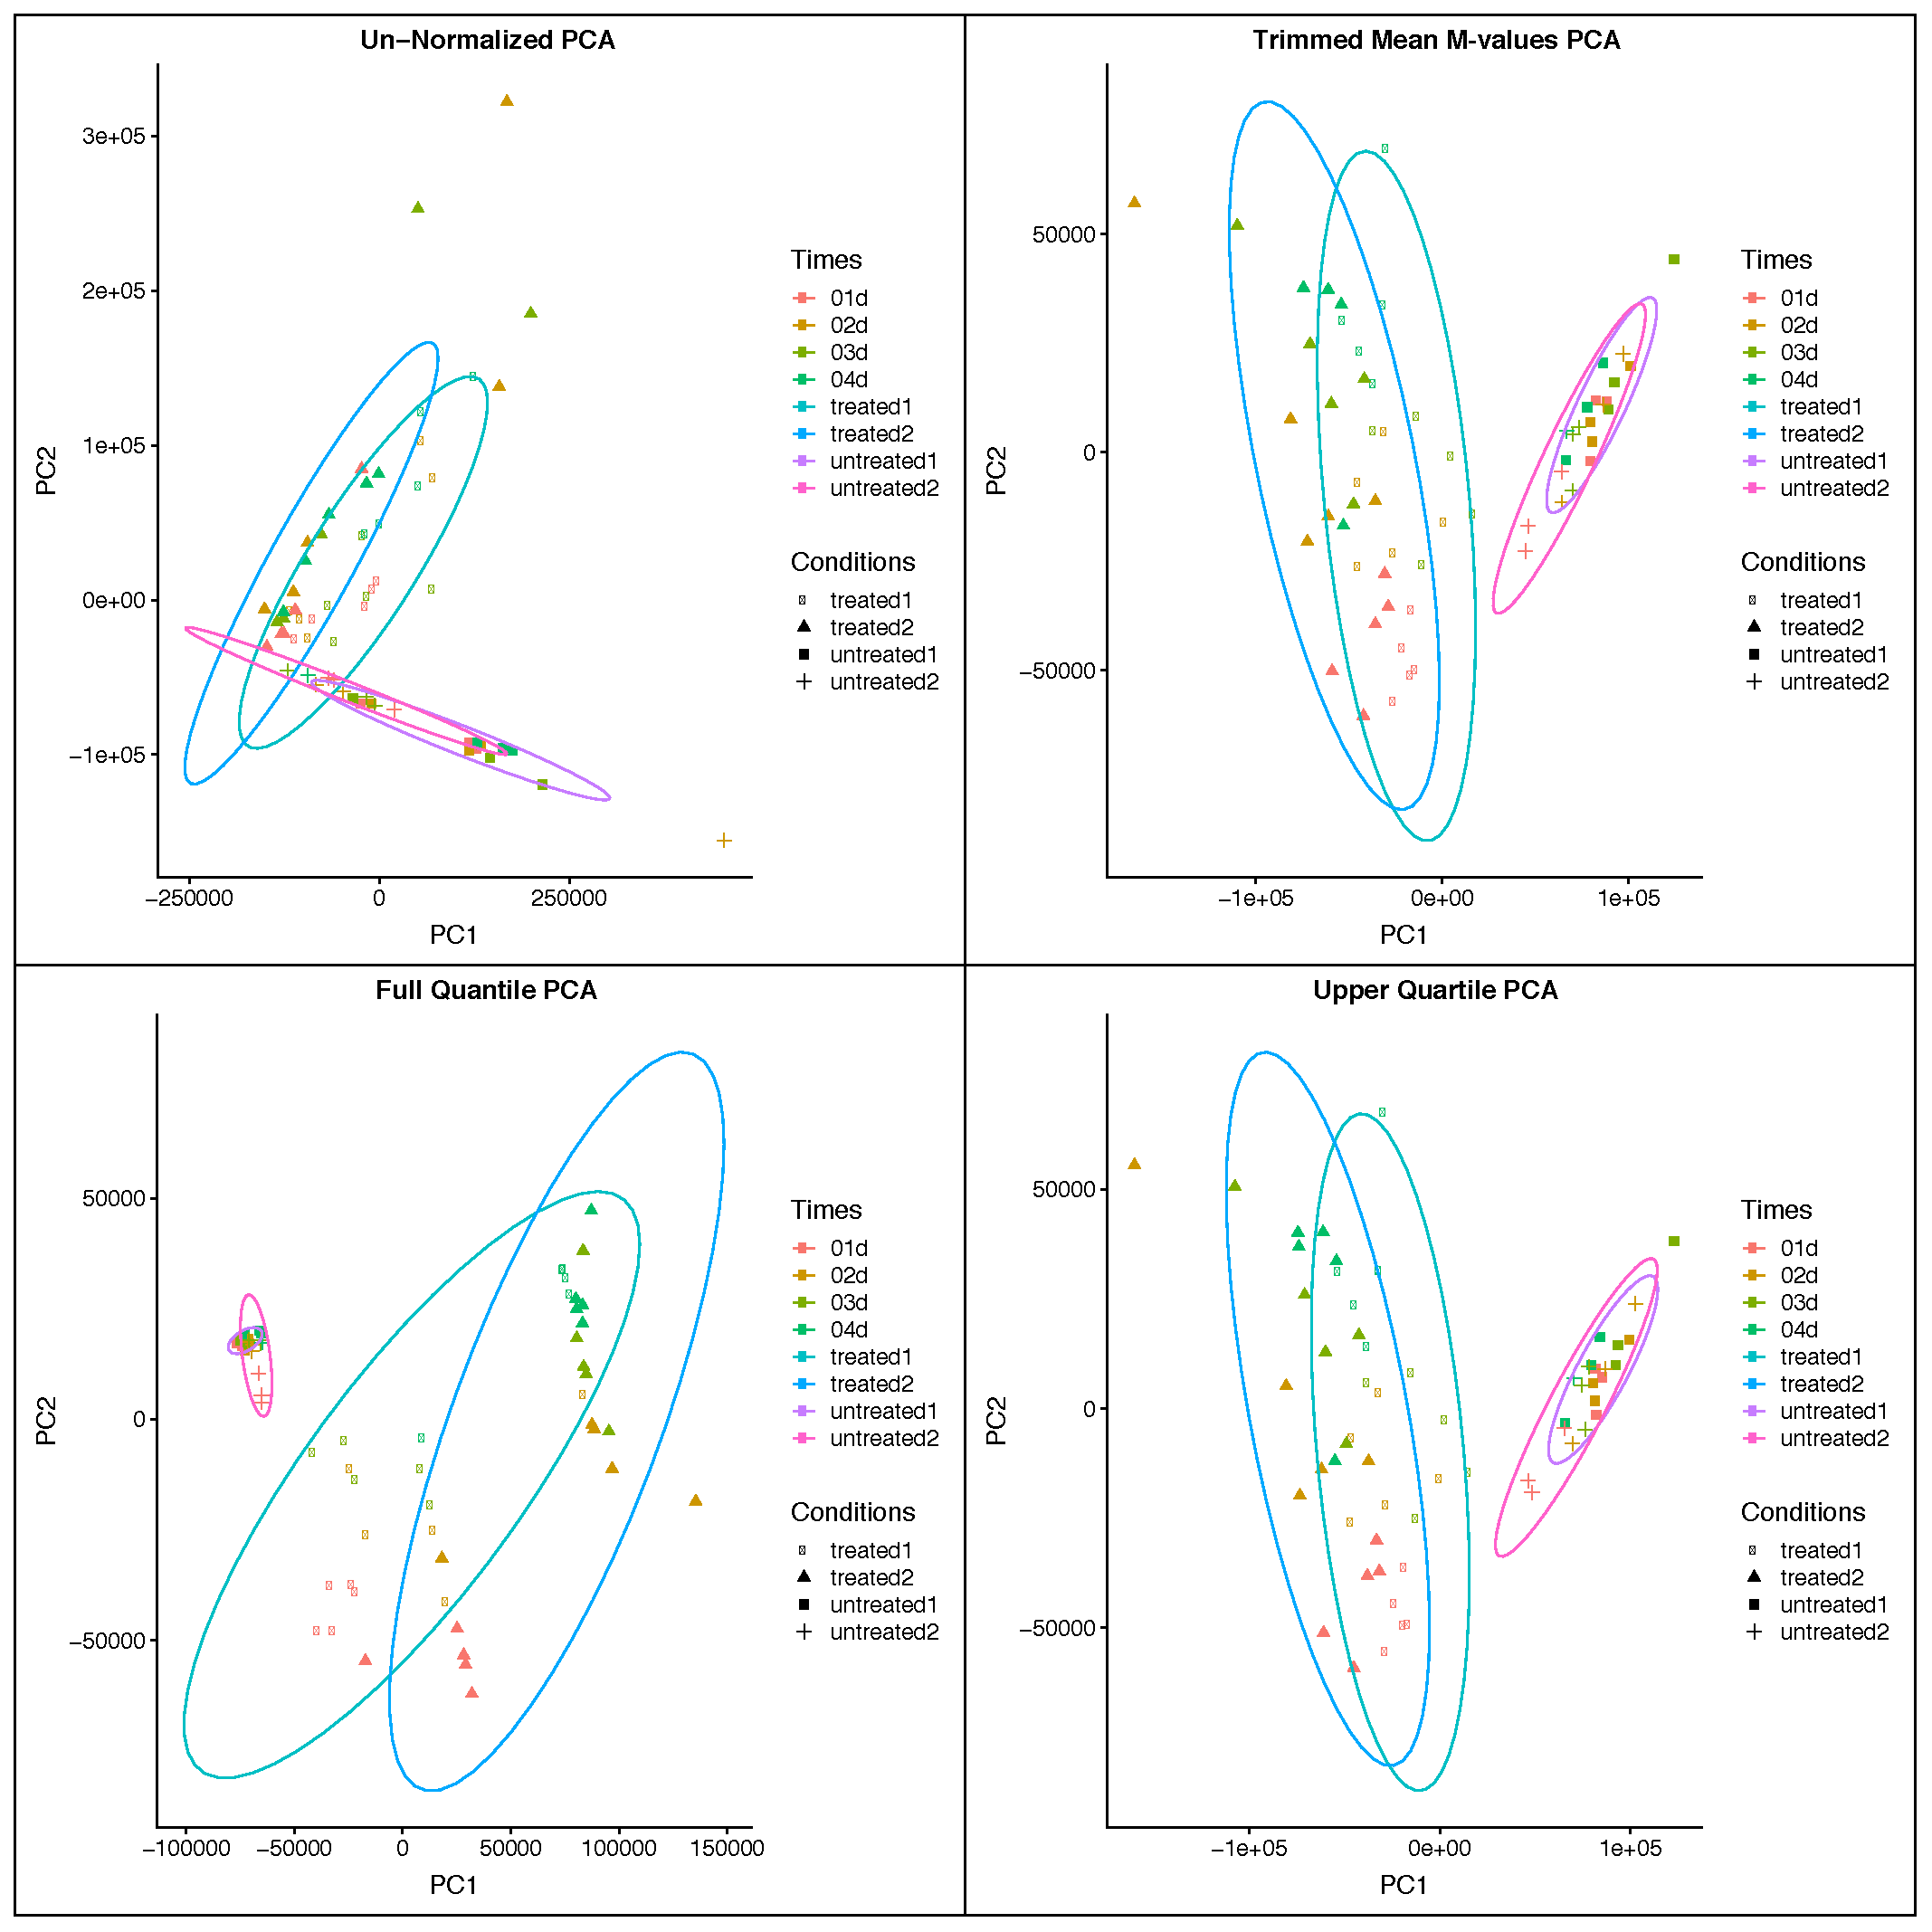
\includegraphics[width=\textwidth,height=\textheight,keepaspectratio]{img/ticorser/normalizing/pca/all_pca.pdf}
\caption[ticorser normalizing methods]{A comparison of how the normalizations methods available in \gls{tic} affect the data.
The first panel shows the clustering of row samples, while the other boxes shows the normalization effect on the samples.}
\label{fig:ticorsernormalizingpca}
\centering
\end{figure}

As already mentioned a boxplot data inspection could not be enough to discriminate between the normalization methods. 
Indeed, looking at the normalized data, as figure \ref{fig:ticorsernormalizingpca} shows, the \textit{TMM} and the \textit{Upper quartile} normalizations are able to well discriminate the treated and the untreated samples, but still preserving some variability inside each group.
While the \textit{Full quantile}, even if it is able to help discriminating the treated and untreated groups, it smashes too much the variability inside the untreated samples.



\subsubsection{Differential Expression}
Once the data are well normalized, in order to be able to well discriminate between the groups, simply by changing our design matrix with only the interested samples, we can focus on the differential expression step.
Here we focus only on half of the total dataset, checking differences between the treated and untreated samples across experimental time points.

For detecting \glspl{deg} across time points taking into account the conditions we designed \gls{tic} with several methods (see section \ref{sec:ticorsermethods} for further details).
Depending on the biological question under investigation, using the \lstinline!ApplyDeSeq2! function and using the count matrix with the design matrix, the package automatically detects the samples to discriminate for the differential expression.
Moreover, depending on the method selected, it is able to detect different types of genes between the samples.
When selecting \lstinline!DeSeqTime_TC! method, it detects all the genes which changes their expression across all time points between two conditions in the \lstinline!Conditions! column of the design matrix, while using \lstinline!DeSeqTime_T!, it recognizes all the genes which have different expression between the conditions across all the time points. 
Furthermore, using \lstinline!DeSeqTime_NoInteraction!, the method is able to detect all those genes demonstrating an oscillating behaviour across the time points in both the conditions.

Additionally, for each of the previous described methods we produce an additional output, obtained with a \textit{Wald Test}, in order to detect all those genes which express differential expression between	the two conditions.

For each method we produce a list of two lists, within the results for the \gls{lrt} and for the \textit{LRT\_Wald}. Each of this already divided for all differential expressed gene, only UP genes, only DOWN genes and the results table with all the genes and their statistics.

Table \ref{tab:ticorserderesults} illustrates differences in catching \glspl{deg} between the three different methods on the same dataset, highlighting the total number of genes reported, with UP and DOWN regulated. 
It is relevant to see that, when applying the \textit{Wald Test} on the results obtained by \gls{lrt} the \glspl{deg} for this test are much higher in number.

\begin{table}[H]
\centering
\begin{tabular}{r c c c c c c c}
%\cline{2-4}\cline{6-8}
%\cline{2-4}\cline{6-8}
\multicolumn{1}{r}{} & \multicolumn{3}{c}{LRT} && \multicolumn{3}{c}{Wald on LRT} \\
%\cline{2-4}\cline{6-8}
\multicolumn{1}{r}{} & Total & UP & DOWN && Total & UP & DOWN \\
\cline{2-4}\cline{6-8}
TC & 825 & 454 & 371 && 7066 & 3606 & 3460 \\
T & 8812 & 4672 & 4140 && 7066 & 3606 & 3460 \\
No-Int & 9560 & 4893 & 4667 && 9567 & 4900 & 4667 \\

\end{tabular}
\caption[\gls{tic} DE methods results]{}
\label{tab:ticorserderesults}
\end{table}


It is also possible to inspect the \textit{DE} results by plotting a \textit{Volcano Plot} or an MA plot, as figure \ref{fig:ticorservolcma} shows.

\begin{figure}[H]
\includegraphics[width=\textwidth,height=\textheight,keepaspectratio]{img/ticorser/de/volcma.pdf}
\caption[ticorser Volcano-MA plots]{}
\label{fig:ticorserfiltering}
\centering
\end{figure}

In order to better compare the results coming from different analysis and methodologies approaches we can use one of the VENN diagrams available in \gls{tic}, which while intersecting the results, saves all the gene lists coming from the intersections and also from exclusions.

\begin{figure}[H]
\includegraphics[width=\textwidth,height=\textheight,keepaspectratio]{img/ticorser/de/venn3.pdf}
\caption[ticorser venn diagram]{}
\label{fig:ticorserfiltering}
\centering
\end{figure}

show plot trends and kegg map





